\documentclass[12pt,a4paper]{article}
\input{stage1.sty}%
% Fichier de style stage2.sty [UTF8]
% Copyleft Laurent Bretonnière, laurent.bretonniere@gmail.com
% Version du 16/03/2015

\usepackage{mathtools}%	
\usepackage{fancybox}%
\usepackage{lastpage}%

\usepackage{fancyhdr}%
\renewcommand{\headrulewidth}{0.8pt}%
\renewcommand{\footrulewidth}{0.8pt}%

\usepackage[tikz]{bclogo}%
\renewcommand\bcStyleTitre[1]{\normalsize\textbf{#1}\smallskip}%
\renewcommand\logowidth{0pt}%

\newcommand{\fin}{\begin{center}%
$\clubsuit\clubsuit\clubsuit$%
\end{center}}%

\newcommand{\un}{\ding{192}\xspace}%
\newcommand{\deux}{\ding{193}\xspace}%
\newcommand{\trois}{\ding{194}\xspace}%
\newcommand{\quatre}{\ding{195}\xspace}%
\newcommand{\cinq}{\ding{196}\xspace}%
\newcommand{\six}{\ding{197}\xspace}%
\newcommand{\sept}{\ding{198}\xspace}%
\newcommand{\huit}{\ding{199}\xspace}%
\newcommand{\neuf}{\ding{200}\xspace}%

\setlength{\headheight}{15pt}%

%*********************************************************************************************
% Cours
%*********************************************************************************************

\usepackage[Lenny]{fncychap}%
\ChNumVar{\fontsize{76}{80}\usefont{OT1}{pzc}{m}{n}\selectfont}%
\ChTitleVar{\raggedleft\Huge\sffamily\bfseries}%

\renewcommand{\thesection}{\Roman{section})}%
\renewcommand{\thesubsection}{\arabic{subsection})}%
\renewcommand{\thesubsubsection}{\alph{subsubsection})}%

%*********************************************************************************************
% Environnements prédéfinis BCLOGO
%*********************************************************************************************

%% Lemme
\newenvironment{lem}{\begin{bclogo}[couleurBord=black!50,arrondi=0.1,logo=\hspace{17pt},barre=none]{Lemme :}}{\end{bclogo}\medskip}%

%% Propriété
\newenvironment{prop}[1][]{\begin{bclogo}[couleur=black!10,couleurBord=black!50,arrondi=0.1,logo=\hspace{17pt},barre=none]{Propriété :~#1}}{\end{bclogo}}%

%% Théorème
\newlength{\textlarg}
\settowidth{\textlarg}{~}
\newenvironment{theo}[1][\hspace{-\textlarg} :]{\begin{bclogo}[couleur=black!5,couleurBord=black!50,arrondi=0.1,logo=\hspace{17pt}, barre=none]{Théorème~#1}}{\end{bclogo}\medskip}%

\newenvironment{theon}[1][]{\begin{bclogo}[couleur=black!5,couleurBord=black!50,arrondi=0.1,logo=\hspace{17pt}, barre=none]{Théorème :~#1}}{\end{bclogo}\medskip}%

%% Corollaire
\newenvironment{coro}[1][]{\begin{bclogo}[couleurBord=black!50,arrondi=0.1,logo=\hspace{17pt},barre=none]{Corollaire :~#1}}{\end{bclogo}\medskip}%

%% Définition(s)

\newenvironment{defi}{\begin{bclogo}[couleur=black!10,couleurBord=black!50,arrondi=0.1,logo=\hspace{17pt}, barre=none]{Définition :}}{\end{bclogo}\medskip}%

\newenvironment{defis}{\begin{bclogo}[couleurBord=black!50,arrondi=0.1,logo=\hspace{17pt}, barre=none]{Définitions :}}{\end{bclogo}\medskip}%

%% Preuve
\newenvironment{pf}{\renewcommand\logowidth{17pt}\begin{bclogo}[noborder=true,logo=\hspace{17pt},couleurBarre=black!25,epBarre=3.5]{Démonstration :}}{\hspace*{\fill}$\Box$\end{bclogo}\smallskip\renewcommand\logowidth{0pt}}%

%\blacksquare

%% Notation
\newenvironment{nota}{\begin{bclogo}[couleurBord=black!50,arrondi=0.1,logo=\hspace{17pt},barre=none]{Notation :}}{\medskip}%

%% Exercice et Exercice-type
\newenvironment{exo}{$\circledast$ \quad\textsc{\underline{exercice} :}~}{\hspace*{\fill}$\circledast$\vskip 8pt}
\newenvironment{type}{$\blacktriangleright$ \quad\textsc{exercice-type :}~}{\hspace*{\fill}$\blacktriangleleft$\vskip 8pt}

%% Exemple(s)
\newenvironment{exem}{\textbf{Exemple :}~}{\medskip}
\newenvironment{exems}{\textbf{Exemples :}~}{\medskip}

%% Remarque(s)
\newenvironment{rem}{\textbf{Remarque :}~}{\medskip}
\newenvironment{rems}{\textbf{Remarques :}~}{\medskip}

%% Rappel(s)
\newenvironment{rap}{\textbf{Rappel :}~}{\medskip}
\newenvironment{raps}{\textbf{Rappels :}~}{\medskip}

%% Cas particulier(s)
\newenvironment{cp}{\textbf{Cas particulier :}~}{\medskip}
\newenvironment{cps}{\textbf{Cas particuliers :}~}{\medskip}

%% Application
\newenvironment{appli}{\textbf{Application :}~}{\medskip}%{\medskip} %
\usepackage[left=1.5cm,right=1.5cm,top=1cm,bottom=1cm]{geometry}
\usepackage{pst-plot,pst-text,pstricks,pst-tree,pstricks-add}
\usepackage{tabularx}
\usepackage{graphicx}



\begin{document}

\pagestyle{empty}
\begin{center}{\LARGE \textbf{\textsc{Fonctions affines (exercices)}}}\end{center}

\textbf{\textsc{\underline{Exercice 1:}}}
\begin{enumerate}
\item Construire, dans le repère de la question /2, les représentations graphiques des fonctions définies par $f(x)=3x-2$, $g(x)=-\frac{3}{4}x+5$, $h(x)=-3$ et $k(x)=2x$.
\item Donner l'expression de chaque fonction associée aux droites suivantes:\\

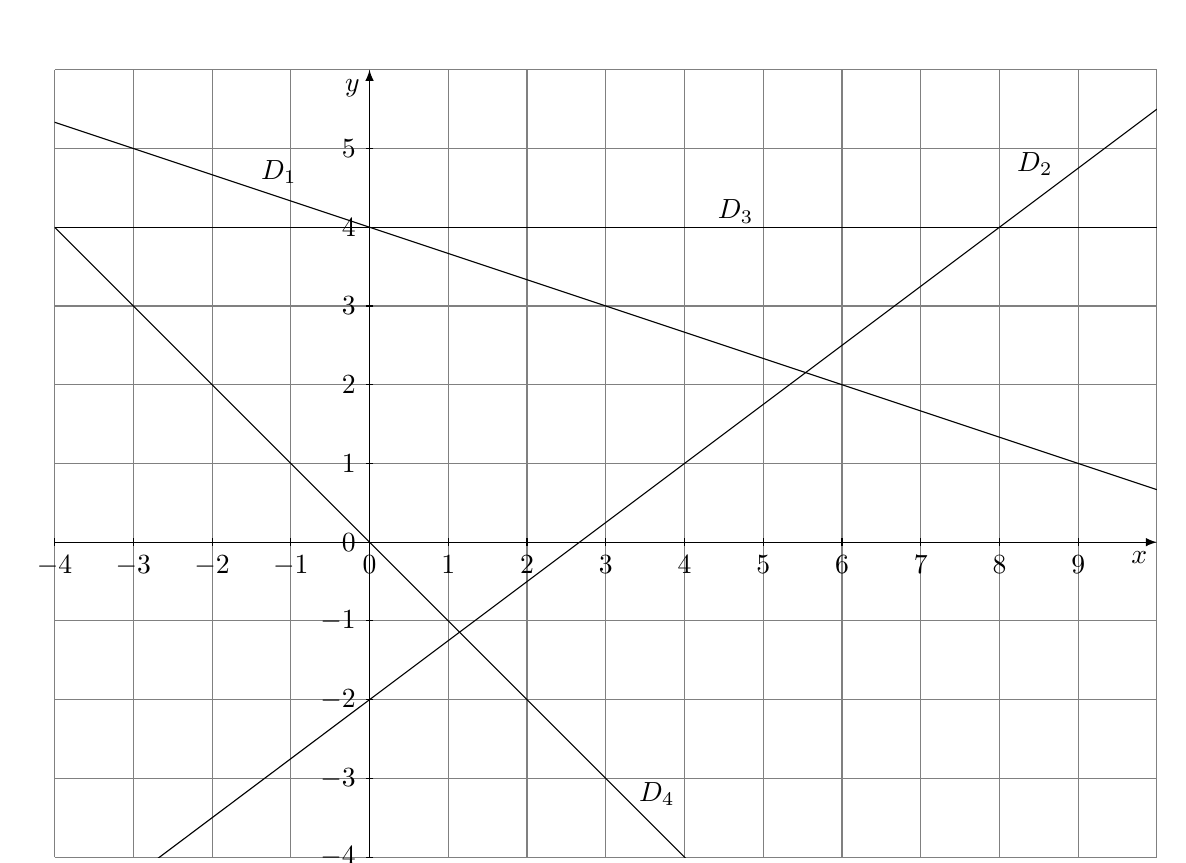
\begin{tikzpicture}[x=10mm,y=10mm]
\draw [gray,xstep=1,ystep=1] (-4,-4) grid (10,6);
\draw [->,>=latex] (-4,0) -- (10,0) node [below left] {$x$};
\draw [->,>=latex] (0,-4) -- (0,6) node [below left] {$y$};

\foreach \x in {-4,...,9}
\draw (\x,0.5mm) -- (\x,-0.5mm) node [below] {$\x$};
\foreach \y in {-4,...,5}
\draw (0.5mm,\y) -- (-0.5mm,\y) node [left] {$\y$};

%\draw (0,0) node [below left] {$O$};

\clip (-4,-4) rectangle (10,6);
\draw [domain=-4:10,samples=100] plot (\x,{-(1/3)*\x+4});
\draw [domain=-4:10,samples=100] plot (\x,{-1*\x});
\draw [domain=-4:10,samples=100] plot (\x,{(3/4)*\x-2});
\draw [domain=-4:10,samples=100] plot (\x,{4});
\draw (-1.5,4.7) node [right] {$\mathscr{D}_{1}$};
\draw (8.1,4.8) node [right] {$\mathscr{D}_{2}$};
\draw (4.3,4.2) node [right] {$\mathscr{D}_{3}$};
\draw (3.3,-3.2) node [right] {$\mathscr{D}_{4}$};
\end{tikzpicture}
\end{enumerate}
\vspace{0,5cm}
\textbf{\textsc{\underline{Exercice 2:}}}\medskip\\
Déterminer l'expression de la fonction affine $f$ telle que $f(-2)=4$ et $f(5)=7$.\\

\textbf{\textsc{\underline{Exercice 3:}}}\medskip\\
Soient $f$ et $g$ les fonctions définies par $f(x)=5x-2$ et $g(x)=\frac{5}{3}x+6$.\medskip
\begin{enumerate}
\item Résoudre l'équation $f(x)=g(x)$. En déduire le point d'intersection entre les courbes $C_{f}$ et $C_{g}$.\medskip
\item Le point de coordonnées $(2;7)$ se trouve-t-il sur la courbe de $f$ ?\medskip 
\end{enumerate}

\vspace{0,5cm}

\textbf{\textsc{\underline{Exercice 4:}}}\medskip
\begin{enumerate}
\item Construire le tableau de signe du produit $(2x-4)(-3x-5)$.\medskip
\item Construire le tableau de signe du quotient $\frac{-3x+9}{7x-5}$.\medskip
\item Donner l'ensemble des solutions de l'inéquation $(2x-4)(-3x-5)<0$ grâce à la réponse à 1/.\medskip
\item Résoudre l'inéquation $\frac{-3x+9}{7x-5}\geqslant0$ grâce à 2/
\end{enumerate}
\vspace{0,5cm}
\textbf{\textsc{\underline{Exercice 5:}}}\medskip\\
Les expressions suivantes définissent-elles une fonction affine ? (justifier et, si oui, préciser le coefficient directeur) :\medskip\\
$f(x)=-5x^2+7x-1$\hfill $g(x)=\frac{3x-5}{7}$\hfill $h(x)=(x-3)(2x-5)-2x^2$


\end{document}